\documentclass{article}
\usepackage[utf8]{inputenc}
\usepackage[document]{ragged2e}

\usepackage{graphicx}
\usepackage{gensymb}
\usepackage{algorithm} 
\usepackage{algpseudocode}


\usepackage[english]{babel}

\usepackage{amsmath}

\usepackage[colorinlistoftodos]{todonotes}

\begin{titlepage}

\newcommand{\HRule}{\rule{\linewidth}{0.5mm}} % Defines a new command for the horizontal lines, change thickness here

\center % Center everything on the page
 
%----------------------------------------------------------------------------------------
%	HEADING SECTIONS
%----------------------------------------------------------------------------------------


\textsc{\Large SOEN6011}\\[0.5cm] % Major heading such as course name
\textsc{\large Deliverable 1 }\\[0.5cm] % Minor heading such as course title

%----------------------------------------------------------------------------------------
%	TITLE SECTION
%----------------------------------------------------------------------------------------

\HRule \\[0.4cm]
{ \huge \bfseries F2: tan(x)}\\[0.4cm] % Title of your document
\HRule \\[1.5cm]
 
%----------------------------------------------------------------------------------------
%	AUTHOR SECTION
%----------------------------------------------------------------------------------------

\begin{minipage}{0.4\textwidth}
\begin{flushleft} \large
\emph{Author:}\\
VIKRAMJIT \textsc{SINGH} % Your name
\end{flushleft}
\end{minipage}
~
\begin{minipage}{0.4\textwidth}
\begin{flushright} \large
\emph{Student ID:} \\
4007577 \textsc{ } % Supervisor's Name
\end{flushright}
\end{minipage}\\[2cm]

% If you don't want a supervisor, uncomment the two lines below and remove the section above
%\Large \emph{Author:}\\
%John \textsc{Smith}\\[3cm] % Your name

%----------------------------------------------------------------------------------------
%	DATE SECTION
%----------------------------------------------------------------------------------------

{\large \today}\\[2cm] % Date, change the \today to a set date if you want to be precise

%----------------------------------------------------------------------------------------
%	LOGO SECTION
%----------------------------------------------------------------------------------------


\includegraphics[width=8cm,height=4cm,keepaspectratio]{images/logo.jpg}\\[1cm] % Include a department/university logo - this will require the graphicx package
 
%----------------------------------------------------------------------------------------

\vfill % Fill the rest of the page with whitespace

\end{titlepage}





\begin{document}


\pagebreak
\tableofcontents
\pagebreak

\chapter{Problem 1}
\section{Introduction}
For real arguments, the Tangent function can defined as: the
tangent of an angle in a right-angle triangle is the ratio of the length of the opposite leg to the length of the adjacent leg.
tan(x) is a periodic tangent function.
Also, Tangent function is basically defined by:

\[ \tan x =  \frac{\sin x}{\cos x}\]









Domain\[(\; \Theta \; , \;\Theta \neq k\frac{\pi}{2}, \;where\; k\; is\; an\; odd\; integer) \]


Co-Domain
\[( -\infty , \infty )\]
\begin{figure}[h!]
  \centering
  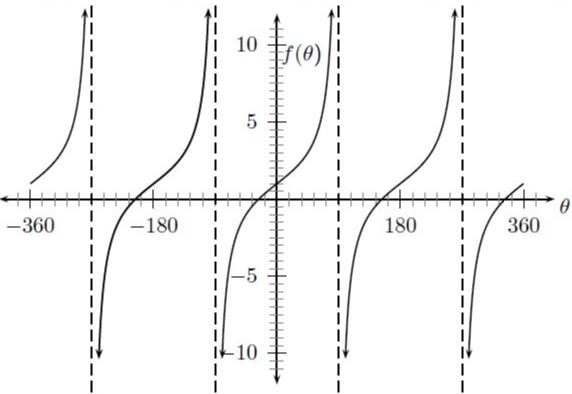
\includegraphics[width=8cm,height=4cm,keepaspectratio]{tan.jpg}
  \caption{$\tan x$}
\end{figure}


\section{Characteristics}
\begin{itemize}
   \item Period of tangent function is \(\pi\). 
   \item Vertical Asymptotes: $x$ = \(\frac{\pi}{2} + k \pi \), where k is an integer. 
   \item Tangent is an increasing function in every interval between any of two successive vertical asymptotes, i.e \(f(x1) < f(x2)\; for\; all\; x1 < x2\). 
   \item Tangent is an odd function with mirror symmetry since \( \tan(-x) = - \tan(x)\) and it’s graph is symmetric with respect to origin. 
   \item  Zeroes of tangent are $n\pi$ for \(n \in Z\), which are same as that of sine function because tangent function will be zero whenever sine function is zero. 
\end{itemize}
\pagebreak
\chapter{Problem 2}
\section{Requirements}
\subsection{First requirement}
\begin{itemize}
\item ID = R1 
 \item Type= Functional Requirement
 \item Version= 1.0
 \item Priority= High 

 \item Description= Value of x can never be \(\pm90^{\circ},\pm270^{\circ},\pm450^{\circ},\pm630^{\circ}\dots\). Function will throw error message if these values are inputted by user.
\end{itemize}
\subsection{Second requirement}
\begin{itemize}
\item ID = R2 
 \item Type= Functional Requirement
 \item Version= 1.0
 \item Priority= High 

 \item Description= If user input anything except numeric value, function will throw error message of wrong input. For Example: If user input string, function will output Wrong Input
\end{itemize}
\subsection{Third requirement}
\begin{itemize}
\item ID = R3 
 \item Type= Functional Requirement
 \item Version= 1.0
 \item Priority= High 

 \item Description= The value of x should be either in degrees or radians.
\end{itemize}
\section{Assumptions}
User always input value of $x$ in \(^{\circ}\) (degree).

\pagebreak
\chapter{Problem 3}
\section{Algorithms}
\subsection{Algorithm 1}
This algorithm uses polynomial approximation to calculate the value of $\tan x$. This Algorithm assumes that user always input x in degrees. Firstly the value of $x$ is reduced to range of  \(-90^{\circ}<x\leq90^{\circ}\). After that Taylor series is applied to x (but before that $x$ is converted to radians)
\subsubsection{Advantages}
\begin{itemize}
    \item Complexity of this algorithm is low.
    \item Through this algorithm, we can find tangent of any angle using only the operations of addition, subtraction, multiplication and division. 
    \item Value of x is reduced to small number using periodicity and symmetry of function, so that the approximations are most accurate.
\end{itemize}
\subsubsection{Disadvantages}
\begin{itemize}
    
    \item Sometimes the calculations become very complex.
    
\end{itemize}

\begin{algorithm}
\caption{ Pseudocode for calculating $\tan x$}

\begin{algorithmic}[1]
\Procedure{$\tan$}{$x$}

\If{($-180>x>180$ )}
  \State $y=|x|/180$
  \If{($x>0$)}
  \State $x=x-y*180 $ 
\EndIf
\If{($x<0$)}
 \State $x=x+y*180 $ 
\EndIf

\EndIf  \Comment{Now,$x$ is in the range of  \(-\ 180^{\circ}<x\leq180^{\circ}\)}

\If{($-90>x>90$ )}
 \If{($x>0$)}
  \State $x=(x-180)$
\EndIf
\If{($x<0$)}
 \State $x=(x+180)$
 \EndIf
\EndIf  \Comment{Now,$x$ is in the range of  \(-\ 90^{\circ}<x\leq90^{\circ}\)}

 \If{$x$ equals to 90 or -90}
  \State print "Math ERROR"
  
\ElsIf{$x$ = 45}
 \State \(tan(x)\) is 1
 \ElsIf{$x$ = -45}
  \State \(tan(x)\) is -1
 \Else
    \State r=\(x*(\frac{\pi}{180}\)) \Comment{Converting degrees to radians }
    \State calculate  \( tan(x)=r+\frac{r^3}{3}+2*\frac{r^5}{15}+17*\frac{r^7}{315}\)
  
\EndIf
 

  

 \EndProcedure \end{algorithmic} 
\end{algorithm}



\pagebreak

\subsection{Algorithm 2}
This algorithm calculates tangent function using the formula \( \tan x =  \frac{\sin x}{\cos x}\). Firstly we calculates the sine of x using Taylor series , than cos of x is calculated using the trigonometric identity \(\sin^2x + \cos^2x = 1\).
\subsubsection{Advantages}
\begin{itemize}
    
    \item Through this algorithm, we can find sine of any angle using only the operations of addition, subtraction, multiplication and division. 
\end{itemize}
\subsubsection{Disadvantages}
\begin{itemize}
    \item The  polynomial approximation is accurate to within \(\pm0.000004\).
   \item Complexity of this algorithm is comparatively high.
   
\end{itemize}

\begin{algorithm}
\caption{ Pseudocode for calculating $\tan x$}

\begin{algorithmic}[1]
\Procedure{$\tan$}{$x$}
\State Calculate $\sin x$
\If{($-360>x>360$ )}
  \State $y=|x|/360$
  \If{($x>0$)}
  \State $x=x-y*360 $ 
\EndIf
\If{($x<0$)}
 \State $x=x+y*360 $ 
\EndIf

\EndIf  \Comment{Now,$x$ is in the range of  \(-\ 360^{\circ}<x\leq360^{\circ}\)}

\If{($-90>x>90$ )}
  \If{($-180>x>180$ )}
    \If{($-270<x<270$ )}
  
 \If{($x>0$)}
  \State $x=(180-x)$
\EndIf
\If{($x<0$)}
 \State $x=(-x-180)$
 \EndIf
 \ElsIf{($-270>x>270$ )}
 \If{($x>0$)}
  \State $x=(x-360)$
\EndIf
\If{($x<0$)}
 \State $x=(360+x)$
 \EndIf
 \EndIf
 \Else
\If{($x>0$)}
  \State $x=(180-x)$
\EndIf
\If{($x<0$)}
 \State $x=(-x-180)$
 \EndIf
\EndIf  \Comment{Now,$x$ is in the range of  \(-\ 90^{\circ}<x\leq90^{\circ}\)}


\If{$x$ = 90}
 \State \(\sin(x)\) is 1
 \ElsIf{$x$ = -90}
  \State \(\sin(x)\) is -1
 \Else
    \State r=\(x*(\frac{\pi}{180}\)) \Comment{Converting degrees to radians }
    \State calculate  \( \sin(x)=r-\frac{r^3}{6}+\frac{r^5}{120}\)
  
\EndIf
\EndIf
\State Calculate $\cos x$
 
\State $\cos x= \sqrt{1-\sin^2x}$
 \State Calculate \( \tan x =  \frac{\sin x}{\cos x}\)
  

 \EndProcedure \end{algorithmic} 
\end{algorithm}
\pagebreak
\subsection{Selection of Algorithm 1}
\begin{itemize}
    \item The Complexity of this algorithm is comparatively less.
    \item The result of this Algorithm is comparatively more accurate.
\end{itemize}


\section{References}
\begin{}{}
\bibitem{link}
\(http://mathonweb.com/help_ebook/html/algorithms.htm#tan\)

\bibitem{link}
\(https://www.siyavula.com/read/maths/grade-11/functions/05-functions-08\)
\end{thebibliography}




\end{document}
